\chapter{Econom\'ia}

Debido a la caracter\'istica meramente investigativa de \'este trabajo, solo
se exponen en este cap\'itulo posibles modelos de negocios alrededor del
\emph{Software Libre}, y algunos nichos de mercado que se encuentran siendo
explotados en la actualidad.\\

\section{Modelos de negocios}
% Contar o cambial la cantidad de categorias, ahora dice 9 pero van a ser mas
La organizaci\'on FLOSSMetrics 
(Free / Libre and Open Source Software Metrics
\footnote{V\'ease - \url{http://www.flossmetrics.org/}})
, que forma parte de la Flossquality (Open source quality research
\footnote{V\'ease - \url{http://www.flossquality.eu/}})
, ambos financiados por la Comisi\'on Europea
\footnote{V\'ease -
\url{http://cordis.europa.eu/fetch?CALLER=PROJ_IST&ACTION=D&RCN=79449}}
, postula varias categorizaciones
\footnote{V\'ease -
\url{http://smeguide.conecta.it/index.php/6._FLOSS-based_business_models}} 
de modelos de negocios potenciales.


%%%%%%%%%%%%%%%%%%%%%%%%%%%%%%%%%%%%%%%%%%%%%%%%%%%%%%%%%%%%%%%%%%%%%%%%%%%%%%%
\subsection{Financiaci\'on externa de empresas}\footnote{En ingl\'es
\emph{Externally funded ventures}}
%
Esta categor\'ia contempla los grupos o compa\~n\'ias que desarrollan
\emph{Software Libre} siendo financiados por una organizaci\'on externa.
Normalmente es esta organizaci\'on externa quien pone las gu\'ias y
requerimientos para el proyecto. Esta categor\'ia es luego desglosada en tres
partes seg\'un el origen de la financiaci\'on.

\subsubsection{Financiaci\'on P\'ublica}\footnote{En ingl\'es \emph{Public
funding}}
%
Se refiere a aquellos proyectos que son financiados por entidades p\'ublicas.
Estos suelen ser proyectos cient\'ificos o desarrollo de est\'andares cuyo
fin
\'ultimo no necesariamente es generar ganancias econ\'omicas si no m\'as bien
alg\'un beneficio social.

\subsubsection{Financiaci\'on ``Necesidad de mejora''}\footnote{En ingl\'es
\emph{``Needed improvement'' funding}}
%
\'Esta es la situaci\'on donde una compa\~n\'ia le paga a un grupo u otro
compa\~n\'ia para que mejore o adapte (y quiz\'a m\'as tarde de soporte) de un
proyecto libre existente.

\subsubsection{Fundaci\'on Indirecta}\footnote{En ingl\'es \emph{Indirect
funding}}
%
Muchas veces ciertas compa\~n\'ias financias proyectos de \emph{Software Libre}
como estrategia de negocio, para obtener, de manera indirecta, alg\'un r\'edito
econ\'omico. El ejemplo m\'as com\'un es cuando un fabricante de
\emph{hardware}
financia a alguien m\'as (muchas veces son sus mismos empleados trabajando
para proyectos de \emph{Software Libre}) para que escriba los \emph{drivers}
para un sistema operativo libre (como lo puede ser GNU/Linux). 

\subsection{Uso Interno}\footnote{En ingl\'es \emph{Internal use}}
%
En este caso, las empresas, optan por realizar un desarrollo propio (en vez,
de quiz\'a, optar por una soluci\'on propietaria ya existente) para solucionar
alg\'un problema en particular. Luego liberan el c\'odigo para beneficiarse de
las contribuciones que puede brindar la comunidad de \emph{Software Libre}.

\subsection{Mejor conocimiento aqu\'i sin limitaciones}\footnote{En ingl\'es
\emph{Best knowledge here without constraints}}
%
En este modelo, una empresa presta servicios como \emph{consultor externo} para
otra compa\~n\'ia sacando r\'edito mediante el alto nivel de conocimiento de su
personal.\
Este tipo de modelos favorece la competencia del mercado, ya que aquella
empresa que necesita consultor\'ia, puede elegir siempre al mejor postor,
obligando a quien provee el servicio a mantener precios competitivos y
asegurar un excelente nivel t\'ecnico en sus empleados.\\

En la provincia de C\'ordoba existen varias empresas que proveen este tipo de
servicios. A continuaci\'on se listan algunas de ellas.

\begin{description}
 \item[Machinalis]\footnote{V\'ease - \url{http://www.machinalis.com/}}
Machinalis provee desarrollo y consultar\'ia de soluciones de calidad basadas
en Software Libre. Desarrollo de aplicaciones web (Python, Django, Zope y PHP).
Soluciones de CMS (Plone y Drupal). Desarrollo de aplicaciones a medida
(Escritorio, Infraestructura, bajo nivel). Uso de metodolog\'ias \'agiles, y
experiencia con trabajo remoto (con clientes hispano y angloparlantes
en todo el mundo). 

\item[Maram Sistemas]\footnote{V\'ease - \url{http://maram.com.ar/}} Soluciones
basadas en Software Libre. Desarrollo de sistemas personalizados. Redes
inal\'ambricas. Servidores web e intranet. Migraciones.

\item[Menttes]\footnote{V\'ease - \url{http://www.menttes.com/}} Productos y
servicios inform\'aticos de alta calidad basados en Software Libre.
 \end{description}

\subsection{Mejor conocimiento aqu\'i con limitaciones}\footnote{En
ingl\'es \emph{Best knowledge here with constraints}}
%
Para prevenir el ``robo'' de clientes, una empresa puede proveer servicios
libres, pero mantener privativo (o con una licencia m\'as restrictiva) a una
peque\~na parte clave c\'odigo.\

Este modelo se puede observar en empresas como Google\footnote{V\'ease -
\url{http://www.google.com/corporate/}} la cual libera gran parte de sus
productos con licencias libres exceptuando algunos productos claves que le
otorgan ventaja competitiva.


\subsection{Doble Licencia}\footnote{En ingl\'es \emph{Dual licensing}}
%
Un modelo muy explotado en el negocio del \emph{Software Libre} es el de doble
licenciamiento. En este modelo la empresa que desarrolla \emph{Software
Libre} otorga licencias libres para los proyectos que vayan a continuar siendo
libres (usualmente entregando el producto gratis) y una licencia distinta
(usualmente paga) para aquellas otras empresas que no deseen redistribuir el
c\'odigo. \\

Los casos m\'as emblem\'aticos de este modelo de negocios son empresas como
\emph{Sun}\footnote{V\'ease - \url{http://www.sun.com}} con su producto
\emph{MySQL}\footnote{
V\'ease - \url{http://www.sun.com/software/products/mysql/getit.jsp}}, el cual
es distribuido con una licencia libre (\emph{GPL}) o bien con una licencia
\emph{comercial} para el caso en el que el comprador no desee redistribuir el
c\'odigo de su producto	.

\subsection{Desarrollo no financiado}\footnote{En ingl\'es \emph{Unfunded
developments}}
%
Existen situaciones donde, si se da con suficiente \'enfasis un efecto de
\emph{networking}\footnote{En castellano \emph{red}. Es cuando por motivos
t\'ecnicos o sociales el proyecto obtiene una impacto importante en 
algunas comunidades de internet.}, requiere solo un esfuerzo m\'inimo de la
organizaci\'on el publicar su producto, ya que la mayor\'ia del aporte lo
obtiene de otras compa\~n\'ias que por diversos intereses asignan recursos
dedicados a ese producto sin pretender un beneficio econ\'omico inmediato.
Los casos m\'as comunes son las distribuciones de GNU/Linux (como
Debian\footnote{\url{http://www.debian.org/}}) o los sistemas operativos
basados en \emph{BSD}\footnote{\url{http://es.wikipedia.org/wiki/BSD}} (como
FreeBSD\footnote{\url{http://www.freebsd.org/}}). Pero el ejemplo m\'as
ilustre de todos es el proyecto
\emph{linux}\footnote{\url{http://www.kernel.org/}}, el cual es desarrollado
por un grupo muy reducido de personas, pero que recibe el aporte de miles de
% 'de alrededor del mundo' o sin el 'de' ????
desarrolladores de alrededor del mundo, muchos de los cuales pertenecen a
diversas empresas y son contratados para \'este trabajo dedicado.
La \emph{Linux Foundation}
public\'o\footnote{\url{
http://www.linuxfoundation.org/publications/whowriteslinux.pdf}} un
art\'iculo\footnote{Que se encuentra algo desactualizado debido a la r\'apida
evoluci\'on de este tipo de proyectos.} donde muestra el aporte de algunas de
las empresas m\'as importantes del mundo al proyecto linux como se puede
observar en la figura \ref{fig:companies_contributions_to_linux}.

% http://www.linuxfoundation.org/publications/images/table4-companies.gif
\begin{figure}[htp]
\centering
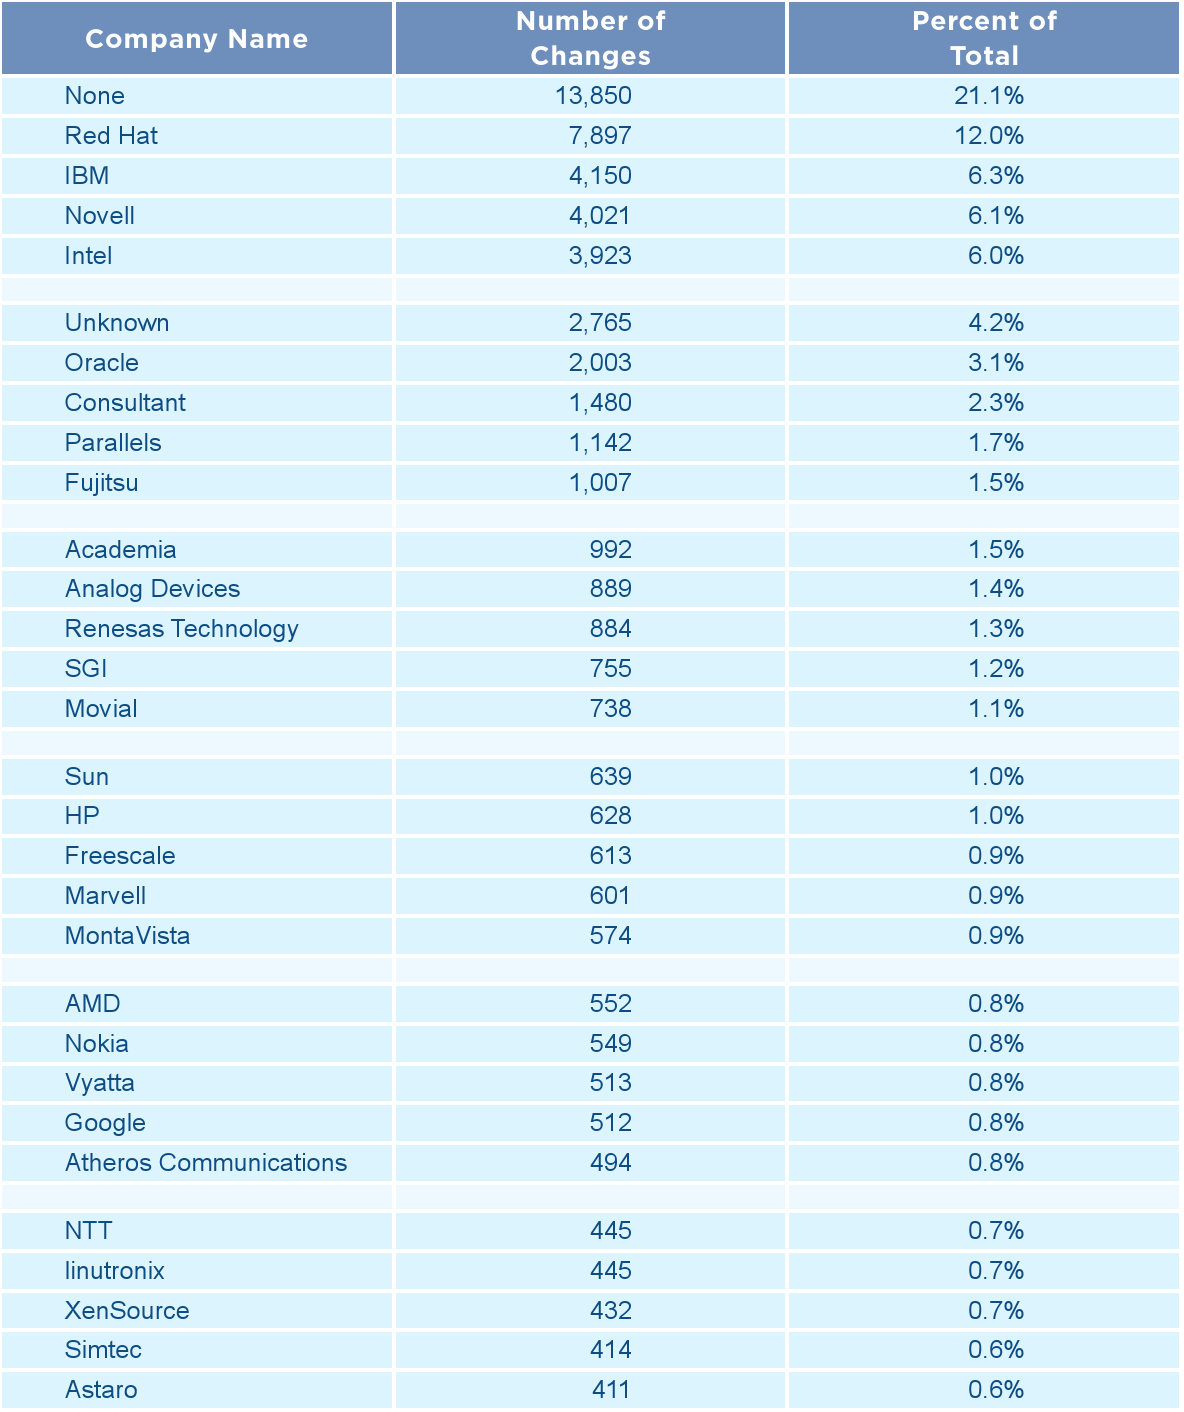
\includegraphics[width=13cm]{./img/table4-companies.png}
\caption{Contribuci\'on de diversas empresas al kernel de linux.}
\label{fig:companies_contributions_to_linux}
\end{figure}\footnote{Datos m\'as actualizados pueden ser generados
autom\'aticamente usando los \emph{scripts} disponibles en
\url{http://www.kernel.org/pub/linux/kernel/people/gregkh/kernel_history/}.}


\section{Posibles modelos particulares}
%
No es el fin de \'este proyecto obtener r\'edito econ\'omico alguno, sin
embargo puede ser de inter\'es de alguien sacar provecho del trabajo aqu\'i
presentado, para ello se analiza a continuaci\'on algunos aspectos
econ\'omicos del mismo.

\subsection{Costos}

Los precios usados son obtenidos de (en caso de ser posible) sus respectivos
fabricantes, o de grandes distribuidores en su defecto, asumiendo compras
mayores de 100 unidades, suponiendo as\'i que es una empresa en vista de
producci\'on en serie quien usar\'a los datos aqu\'i presentados.\\

% PIC18F4550 = 4.26 USD
% http://www.microchipdirect.com/productsearch.aspx?Keywords=18f4550

% Conector USB B hembra = 0,37 €
% http://es.farnell.com/lumberg/2411-02/hembra-usb-panel-pcb-tipo-b/dp/1177885

% TIP 122 = 0,33 € 
%http://es.farnell.com/multicomp/tip122/transistor-darlington-to-220/dp/9294236

% PCB ~= 2 o 3 USD
% pcbcart.com

% 3 USD extra
% Diodos, transistores, resistencias, optoacopladores y conectores.

Al ser un dise\~no sencillo, solo hay algunos elementos claves del mismo que
poseen valor comparable al total.\ 
La tabla \ref{tab:element_cost} muestra los precios unitarios de estos
elementos.


\begin{table}[ht]
\centering
\begin{tabular}{r|l}
Elemento    & Precio (USD) 	\\ \hline
PIC18F4550  & 4.26			\\
Ficha USB   & 0.52			\\
TIP122      & 0.47			\\
PCBs        & 2				\\
Extras		& 3				\\
\end{tabular}
\caption{Precios unitarios por cien unidades} 
\label{tab:element_cost}
\end{table}


Luego por unos diez dolares es posible armar ambas placas, y gracias a haber
elegido todo software libre para el desarrollo, no es necesario comprar ninguna
herramienta que agregue costo extra al dispositivo.\\

\subsection{Modelos de negocio}

Las caracter\'isticas particulares de este trabajo permite trabajar con varios
modelos distintos.\\

Es importante notar que este trabajo se encuentra completamente liberado, por
lo que cualquier interesado puede usarlo sin pagar nada, y todas las
especificaciones del mismo tambi\'en pueden obtenerse sin costo alguno. \
No obstante los siguientes modelos son perfectamente aplicables, y pueden ser
transferidos durante todo la cadena del mercado.\\


\begin{description}
 \item[Venta de soporte] Quien posea el conocimiento t\'ecnico del desarrollo
puede vender soporte, a alg\'un potencial cliente que desee productizar el
trabajo. 

 \item[Venta de paquete de desarrollo] Es posible empaquetar todo el trabajo de
tal manera de entregarle al cliente una distribuci\'on de GNU/Linux con todas
las herramientas necesarias instaladas para comenzar la productizaci\'on sin
tener que preocuparse por configurar el ambiente de desarrollo. 

 \item[Venta de desarrollo particular] Si el cliente desea alguna
funcionalidad extra que actualmente no ese encuentra implementada o quiz\'a
portar el c\'odigo a otro sistema operativo, el trabajo de desarrollar e
implementar los requerimientos puede venderse.
\end{description}

Otro tema importante a notar es que la licencia usada (GPL v3) fuerza a que
toda obra derivada de este trabajo mantenga la misma licencia y sea publicada,
por lo que cualquier mejora hecha al mismo, ya sea pagada por un cliente
privado o sencillamente implementada por un particular, siempre se har\'a
p\'ublica.




